
\chapter{Finding Minima of Neon Replacements}
\label{chap:Erstes Kapitel}
\section{Neon interaction LAMMPS setup}
-potential curves for na-ne, na-na, ne-ne interactions\\
-explain setup of calculation with ball being carved out\\
-maybe here explain the nearest neighbours
\section{Sodium Monomer}
-Not feasible to brute force dimer with 3rd nearest neighbors\\
-explain nearest neighbors\\
-even with full 48 cubic point symmetry of the host of the defect which no structure can exceed ...\\ 
-explain confirmation of algorithm with brute force for mono sodium\\
-explain how plot is created with sweeps\\
-more complicated symmetries\\
-compare figures\\
-calculation for dimer\\
-discuss noteworthy structure (e.g. inner shell carved out)\\
-citation of paper that has the same plot
Now first by brute force search we know the minima for a single sodium atom.

%\begin{figure}[h!]
%	\centering
%	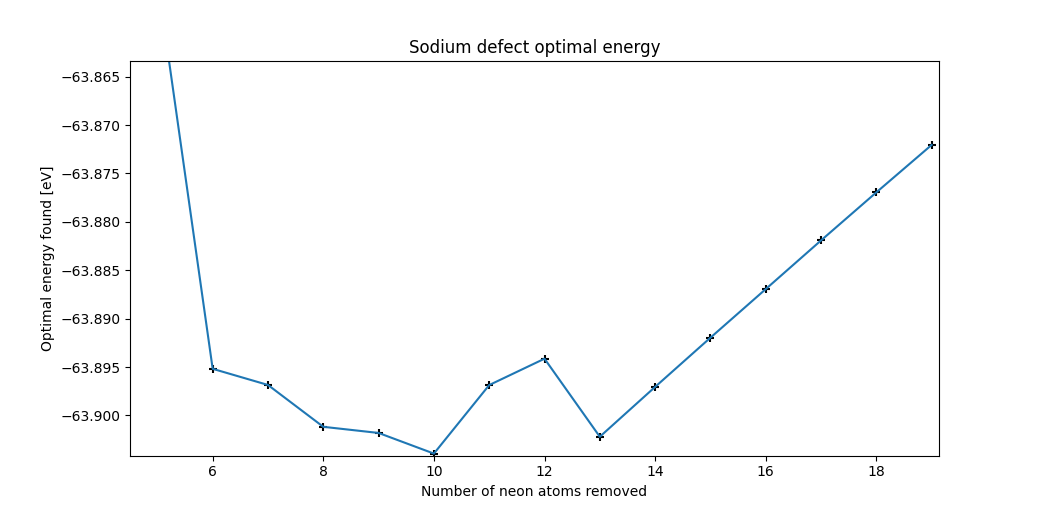
\includegraphics[scale=0.5]{./Inhalt/Bilder/optimal_defect_brute_force.png}
%	\caption{Brute force for single sodium atom}
%	\label{fig:bruteforcesodium}
%\end{figure}

\begin{figure}[h!]
	\centering
	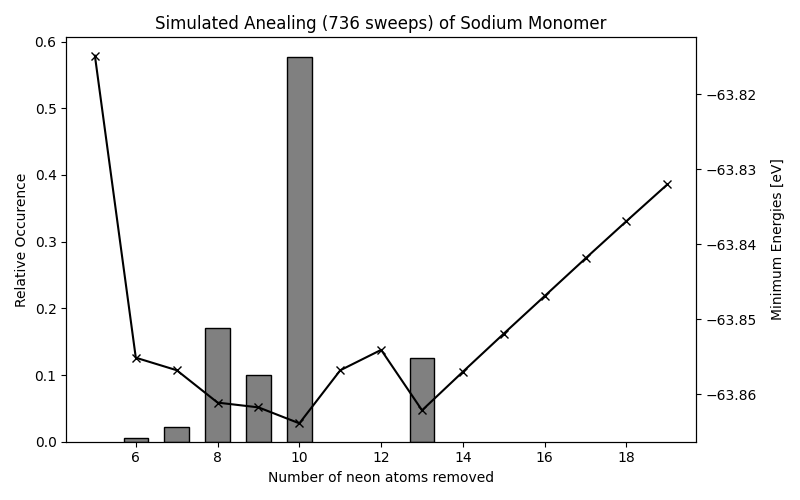
\includegraphics[scale=0.5]{./Inhalt/Bilder/optimal_defect_simulated_annealing.png}
	\caption{Simulated Annealing for single sodium atom inserted, compared to a brute force minima search for a fixed number of removed atoms S.}
	\label{fig:simulatedannealingsodium}
\end{figure}  

So \ref{fig:simulatedannealingsodium} shows the simulated annealing algorithm accurately icks up on the location of the minima, albeit with no quantitative measure misleading local minima being blown out of proportion (See S=8).

\section{Sodium Dimer}
-3rd nearest neighbors, why ? because minima is more the 2 shells
-rough estimate of time used by brute forcing\\
-even with full cubic symmetry this is too long (divide b 64)\\
-maybe think about symmetry\\
-same graphics as for the monomer case\\
-heuristically take the maxima of these plots \\
-give structures\\
-discuss structures (inner shell carved out)\\

\begin{figure}
	\centering
	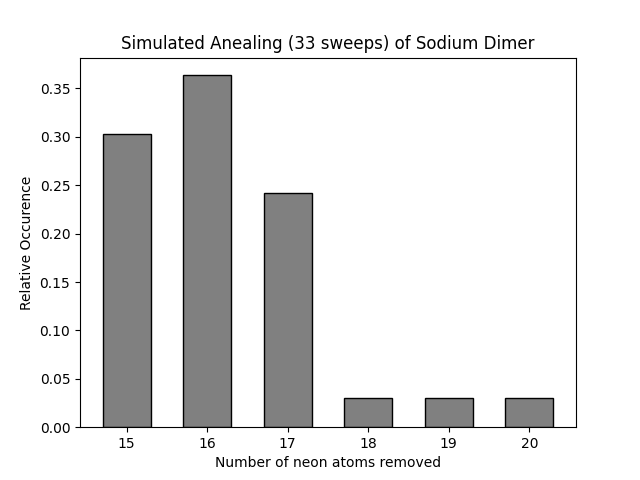
\includegraphics[scale = 0.5]{Inhalt/Bilder/optimal_defect_simulated_annealing_dimer.png}
	\caption{Simulated annealing results and their relative occurrence after 33 sweeps}
	\label{fig:simulatedannealingsodiumdimer}
\end{figure}

\chapter{DFT optical spectra results}
\label{chap:Zweites Kapitel}
%
Zweites Kapitel
%
%
\chapter{Conclusion}
Unfortunately no confidence or error can be estimated since the approach was purley heuristcal. Optical spectrum does not depend much on replacements and precise structure.



